\documentclass[conference,onecolumn,letterpaper,romanappendices,12pt,english,nofonttune]{IEEEtran}
\IEEEoverridecommandlockouts
\usepackage[margin=1in]{geometry}
\usepackage{setspace}
\usepackage[compact]{titlesec}
 \titlespacing{\title}{0pt}{0pt}{24pt}
 \titlespacing{\section}{0pt}{10pt}{6pt}
 \titlespacing{\subsection}{0pt}{*0}{*0}
 \titlespacing{\subsubsection}{0pt}{*0}{*0}
 \titlespacing{\appendix}{0pt}{*0}{*0}

\renewcommand{\appendix}{}

\usepackage[runin]{abstract}
 \renewcommand{\abstractnamefont}{\normalfont\normalsize\itshape}
 \renewcommand{\abstracttextfont}{\normalfont\normalsize}
 \setlength{\absleftindent}{0mm}
 \setlength{\absrightindent}{0mm}
 \abslabeldelim{--}

\usepackage{lastpage}
\usepackage{fancyhdr}
 \setlength{\headheight}{0.6in}
 \setlength{\headsep}{15pt}
 \setlength{\voffset}{-0.5in}
 \renewcommand{\headrulewidth}{0pt}
 \renewcommand{\footrulewidth}{0pt}
 \fancyhf{}
 \fancyfoot[C]{\thepage\ of \pageref{LastPage}}
 \pagestyle{fancy}

\usepackage[ngerman,main=english]{babel}
\usepackage{xcolor}
\usepackage[pdftex]{graphicx}
\usepackage{wrapfig}
\usepackage{newtxtext,newtxmath}
\usepackage[group-minimum-digits=4,per-mode=fraction]{siunitx}
\usepackage[T1]{fontenc}
\usepackage{caption}
	\captionsetup[table]{labelsep=period,font=small,font=sc}
	\captionsetup[figure]{font=small,justification=centerlast}
\usepackage{subcaption}
\usepackage{booktabs}
\usepackage{enumitem}
\usepackage{soul}
\usepackage[noadjust]{cite}

\usepackage[capitalize,noabbrev]{cleveref}
 \crefname{figure}{Fig.}{Figs.}
 \crefname{equation}{Eq.}{Eqs.}
 \crefname{section}{Section}{Sections}
 \crefname{table}{Table}{Tables}

\usepackage{multirow}
\renewcommand{\IEEEbibitemsep}{6pt}
\makeatletter
\IEEEtriggercmd{\reset@font\normalfont\fontsize{12pt}{12pt}\selectfont}
\makeatother
\IEEEtriggeratref{1}

\graphicspath{{./figures/}}
\hyphenation{op-tical net-works semi-conduc-tor}

\begin{document}
 \bstctlcite{bstctl:etal, bstctl:nodash, bstctl:simpurl}

\title{Hardware-Algorithm Co-Design of an Action-Regularized DRL Controller for DC-DC Converters}
% AUTHOR INFO REMOVED FOR DOUBLE-BLIND REVIEW
\author{}
\maketitle
\vspace{-0.5in}
\thispagestyle{fancy}
\setstretch{1.2}

\begin{abstract}
\normalsize
Deep reinforcement learning (DRL) presents a viable control paradigm for DC-DC converters facing nonlinear variations. However, application to high-frequency power electronics is hindered by control chattering and prohibitive inference latency. This digest proposes a hardware-algorithm co-design framework achieving cycle-by-cycle DRL control for a 1 MHz, 12 V to 5 V step-down converter. Algorithmically, a Proximal Policy Optimization (PPO) agent leverages an action-regularized reward to suppress steady-state voltage ripples. The hardware implementation features a fully pipelined fixed-point neural network synthesized on a Zynq-7000 FPGA. Integrated with a custom 4-phase DPWM, state quantization and network inference execute within a sub-microsecond window. Validation confirms robust transient recovery, demonstrating the capability of artificial intelligence to govern high-frequency converters under strict temporal constraints.
\end{abstract}

\vspace{0.2\baselineskip}
\noindent\textbf{\textit{Keywords-}}
\textbf{\textit{DC-DC converters, deep reinforcement learning, FPGA hardware acceleration, Proximal Policy Optimization, DPWM}}

\renewcommand{\baselinestretch}{1.5}\normalsize

\section{Introduction}

Intermediate 12 V to 5 V bus converters demand tight transient responses under rapid load shifts. Although traditional linear controllers and model predictive control (MPC) are industry standards, they often require extensive mathematical modeling and exhaustive tuning to handle severe non-linearities, such as continuous to discontinuous conduction mode (CCM/DCM) transitions. Deep reinforcement learning (DRL) \cite{gheisarnejad2020iot, ye2024deep} offers a compelling data-driven alternative; however, its high-frequency integration remains challenging. Unconstrained DRL policies induce high-frequency action chattering, increasing voltage ripples and threatening system stability \cite{11106282}. Furthermore, standard software-based neural network execution typically incurs tens of microseconds of latency. This fundamentally prevents \SI{1}{MHz} cycle-by-cycle tracking, confining DRL to low-frequency applications or slow outer-loop tuning \cite{11040024, zeng2023deep}.

To overcome these limitations, an ultra-low-latency, action-regularized FPGA DRL controller is presented. The classical 12 V to 5 V step-down converter is deliberately selected as a canonical benchmarking vehicle. By utilizing this well-understood topology, the validation effectively isolates and demonstrates the pure computational feasibility of sub-microsecond DRL execution, decoupled from the cross-dynamics of complex multi-variable converters. The proposed approach integrates a Proximal Policy Optimization (PPO) algorithm optimized to penalize jitter, a custom fixed-point hardware neural network formulated to ensure sub-microsecond inference, and a 4-phase DPWM core implemented to prevent quantization-induced limit cycles, thereby achieving robust cycle-by-cycle artificial intelligence control at \SI{1}{MHz}.

\begin{figure}[t]
	\centering
	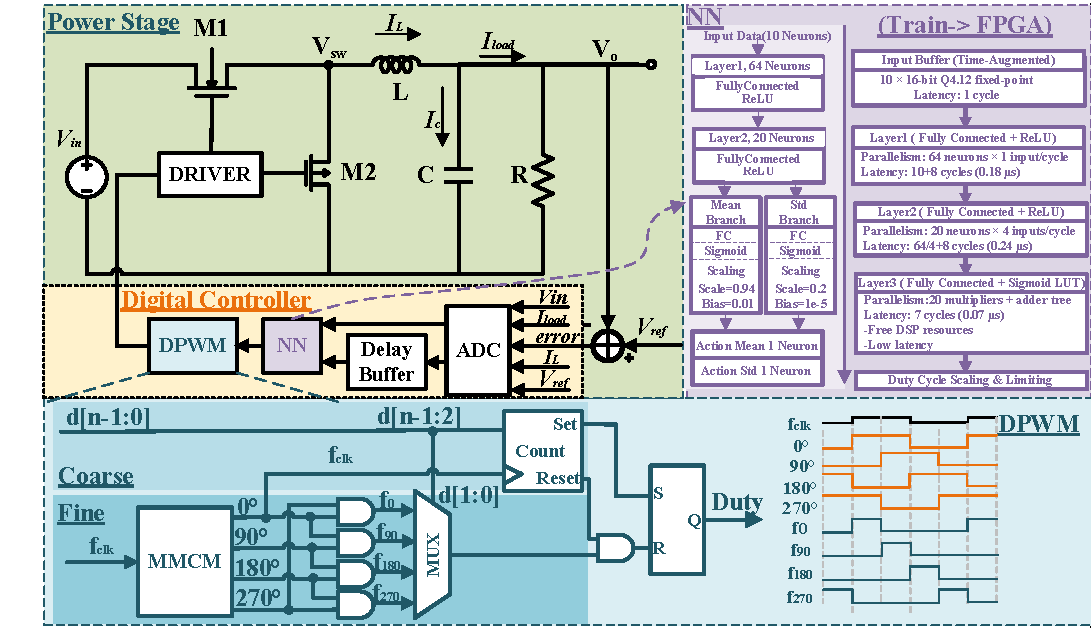
\includegraphics[width=\linewidth]{figures/mea434.pdf}
	\caption{Top-level hardware-algorithm co-design architecture of the DRL-controlled DC-DC converter.}
	\label{fig:top_arch}
\end{figure}

\section{Hardware-Algorithm Co-Design}

\subsection{Robust State Extraction and Regularized PPO}
To regulate the converter independently of static parameters, a 10-dimensional sequential state space encodes temporal dynamics via current and delayed samples: $\mathbf{obs}(t) = [\mathbf{x}(t), \mathbf{x}(t-1)]^T$, where $\mathbf{x} = [v_{\text{in}}, i_L, i_{\text{out}}, v_{\text{ref}}, e]$. This delay embedding mitigates non-Markovian dynamics by implicitly approximating $di/dt$ and $dv/dt$. Hardware preprocessing utilizes an asynchronous FIFO to bridge the ADC and control domains, underflow-proof logic for bias removal, and noise clamping. The preprocessed vector is mapped to a Q4.12 fixed-point format and latched into the neural network at the \SI{1}{MHz} control rate.

The PPO agent outputs a continuous action bounded to $a \in [0.01, 0.95]$ to prevent duty-cycle saturation. To enforce steady-state smoothness, rapid action variations ($e_{action} = a_t - a_{t-1}$) are penalized by the reward function (\cref{eq:reward}) to regularize against high-frequency jitter:
\begin{equation}
 \label{eq:reward}
 R_t =
 \begin{cases}
 -k_1 \sqrt{\left| e_{norm} \right|} - k_2 |e_{action}| & \text{if } |e_{norm}| < 0.01 \\
 -k_3 \sqrt{\left| e_{norm} \right|} & \text{otherwise}
 \end{cases}
\end{equation}
\noindent
where $e_{\text{norm}} = e_t / V_{\text{ref}}$, $k_1 = 1$, $k_2 = 5$ and $k_3 = 10$.

\subsection{Ultra-Low Latency Inference and 4-Phase DPWM}
The 10-64-20-1 MLP policy is synthesized into a hardware accelerator (\cref{fig:top_arch}). A Time-Division Multiplexing (TDM) strategy minimizes hidden-layer footprint, while a 5-stage unbalanced binary addition tree processes the output layer to prevent pipeline stalls. Sigmoid activations utilize BRAM look-up tables. With Q4.12 fixed-point arithmetic, inference completes within 60 clock cycles ($< 0.6~\mu\text{s}$ at \SI{100}{MHz}). Offline profiling confirmed a negligible Q4.12 mean squared error ($<10^{-8}$). Hardware-level validation verified near-exact action fidelity against the floating-point baseline. The target action drives a custom 4-phase DPWM, utilizing 7 MSBs for coarse thresholds and 2 LSBs for exact phase shifts, ensuring continuous mapping.

\begin{figure}[t]
	\centering
	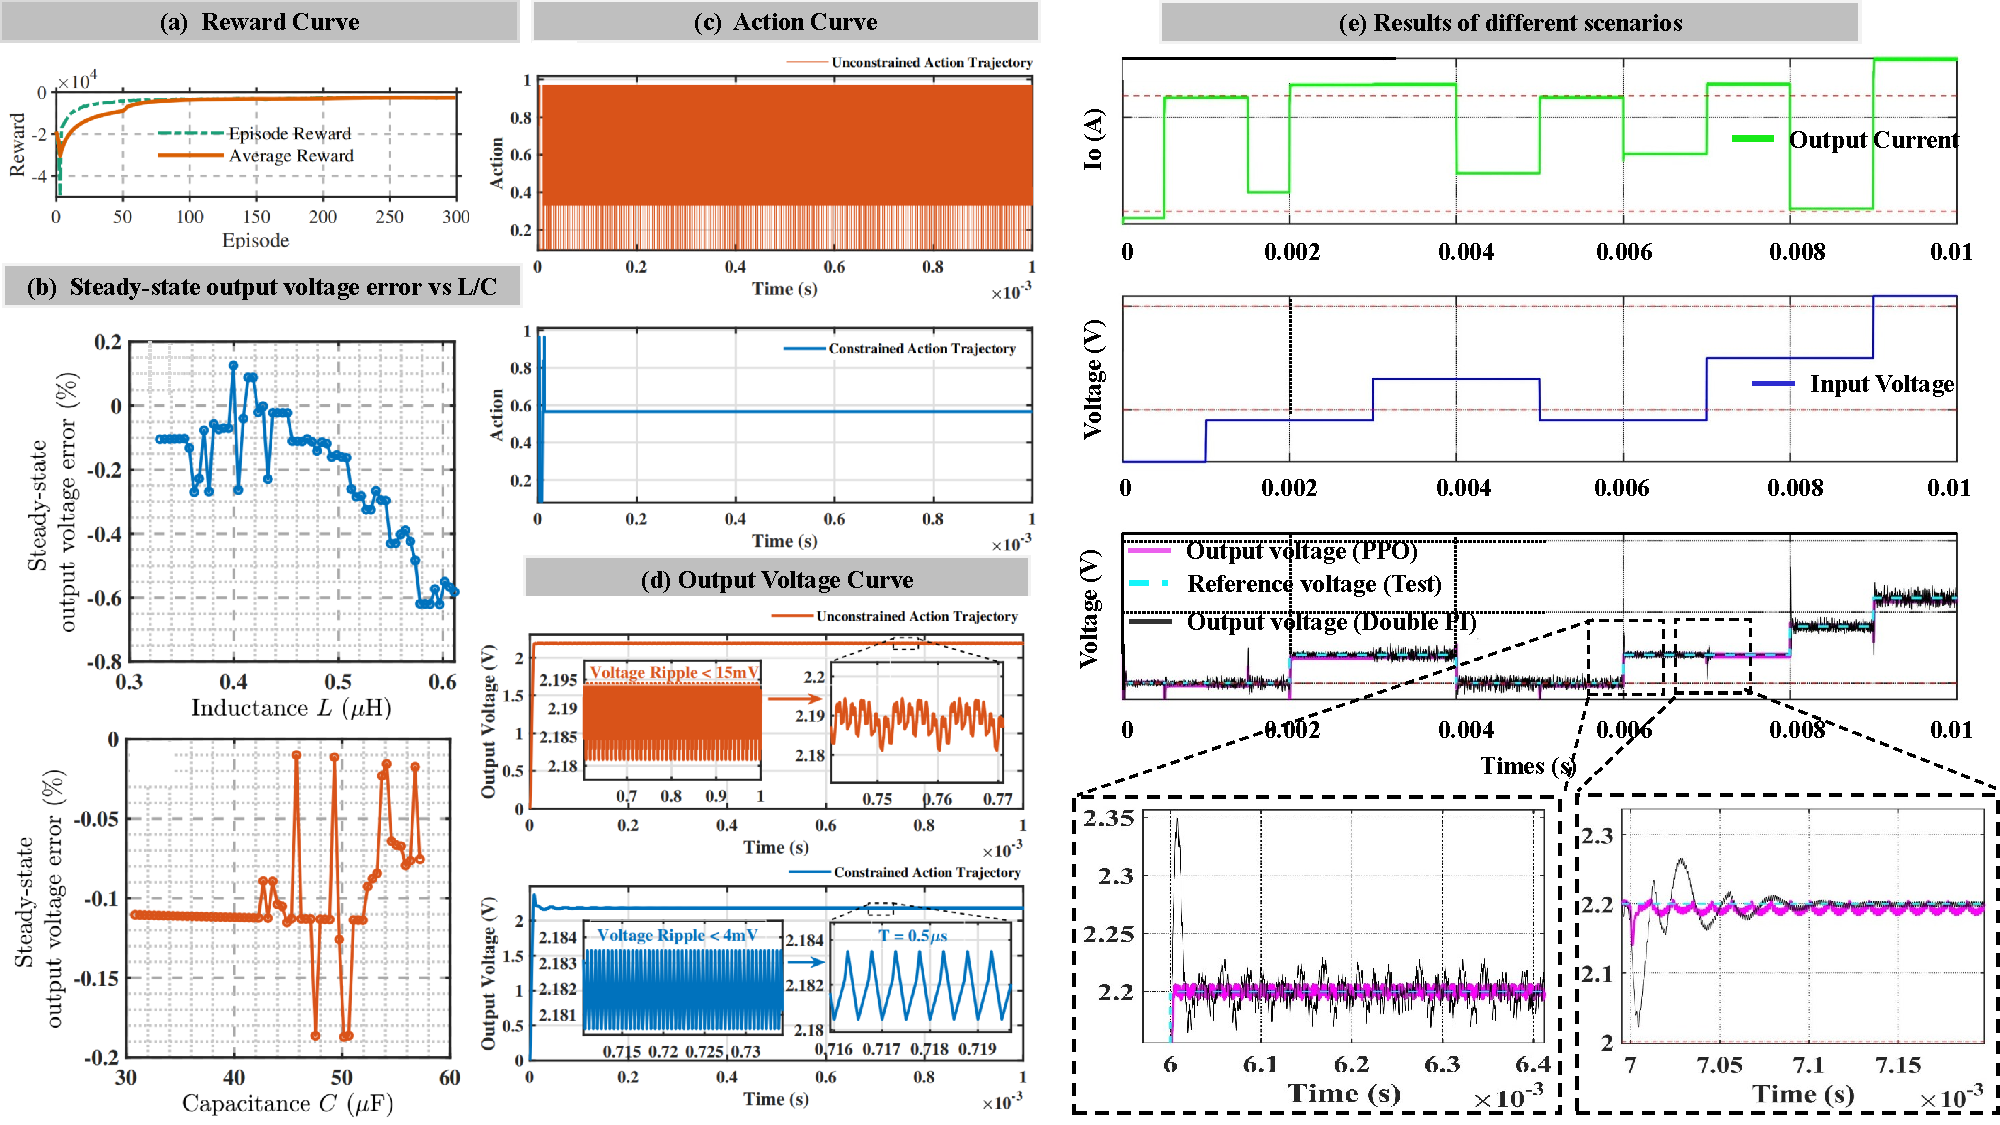
\includegraphics[width=\linewidth]{figures/simulation2.pdf}
	\caption{Algorithmic and comparative simulation performance: (a) Reward curve; (b) Steady-state error distribution under component tolerances; (c)-(d) Action trajectory and output ripple suppression via regularized reward; (e) Transient and steady-state comparison between the proposed PPO and a high-bandwidth Double PI controller.}
	\label{fig:measurement}
\end{figure}


\begin{figure}[t]
	\centering
	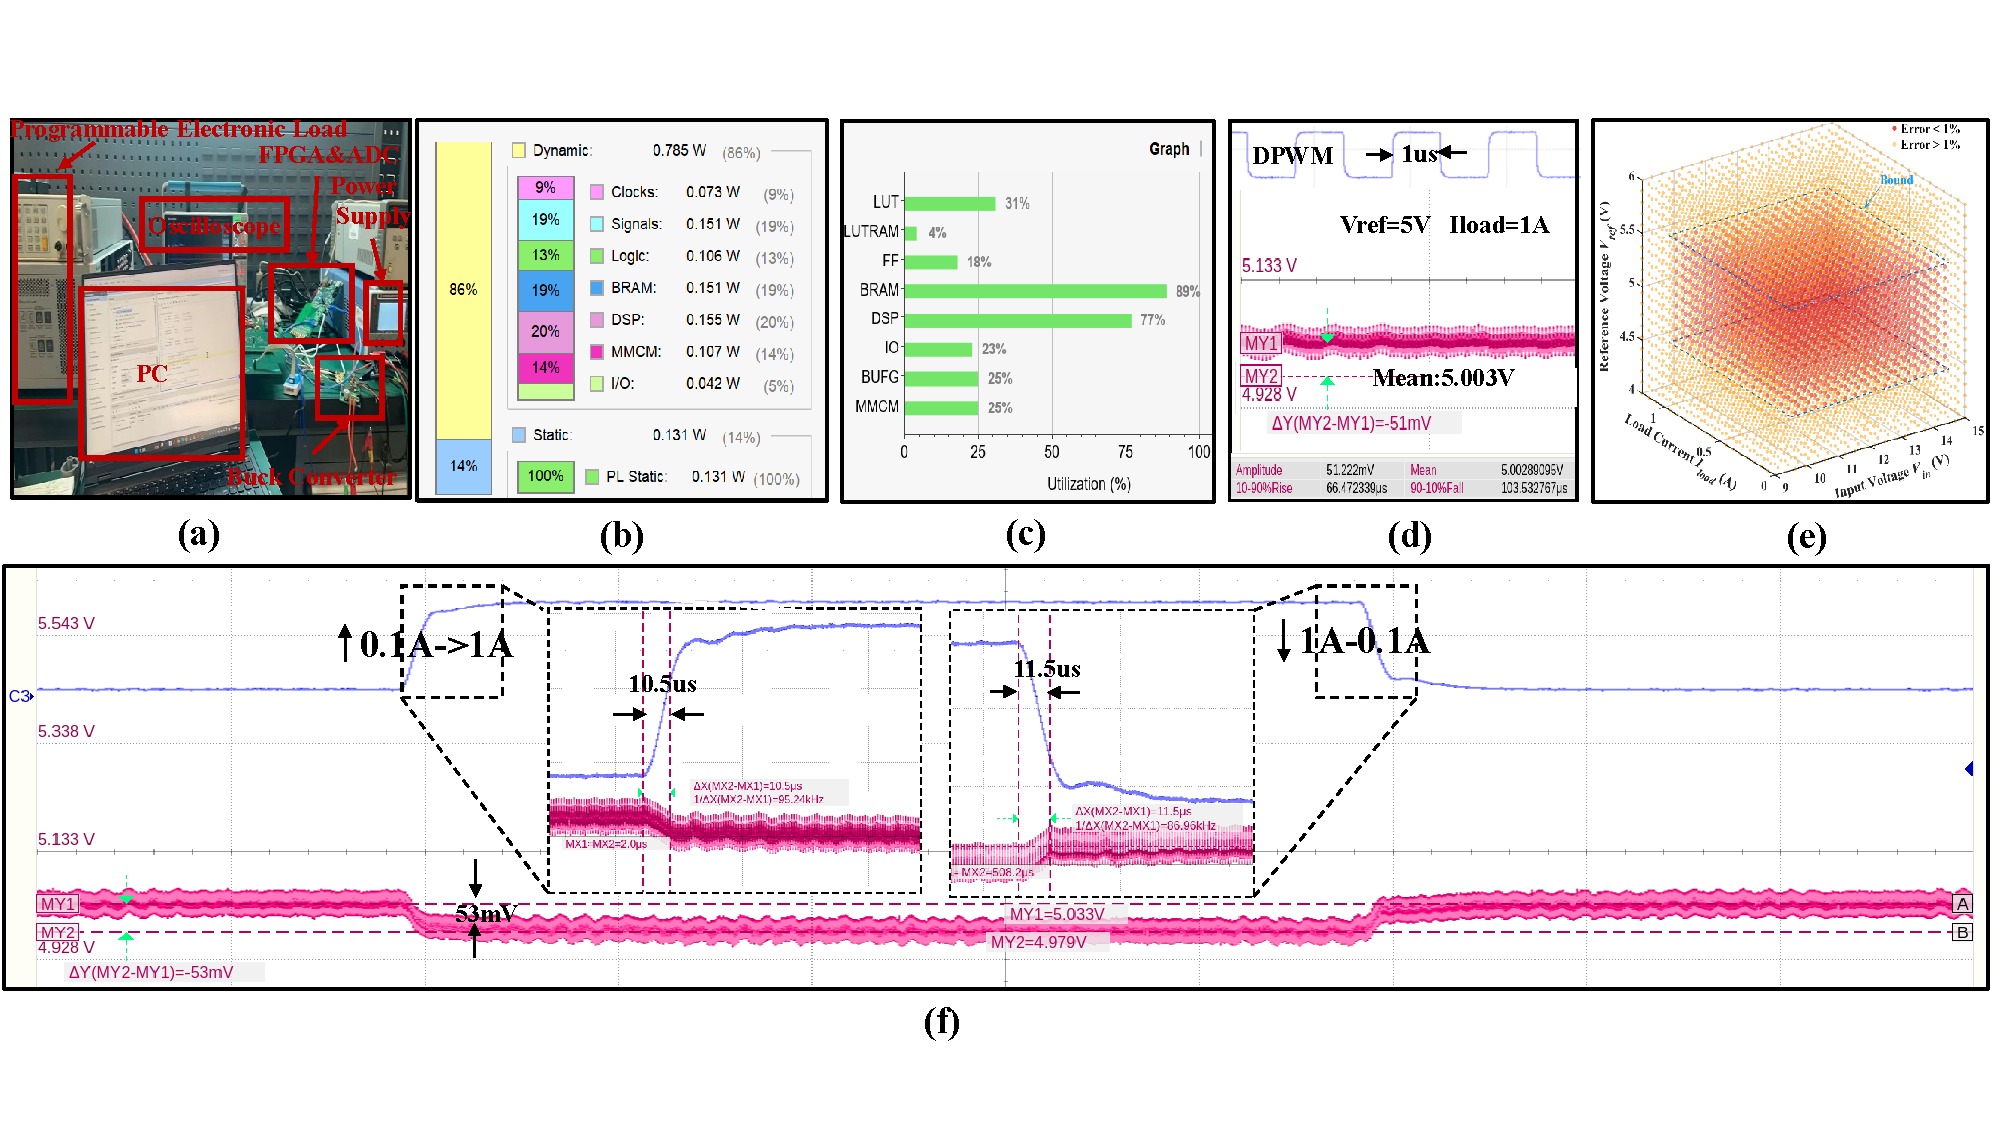
\includegraphics[width=\linewidth]{figures/MEASURE555.pdf}
	\caption{Hardware measurement results: (a) Experimental setup; (b)-(c) FPGA power and resource utilization; (d) Steady-state execution latency; (e) Steady-state response performance; (f) Dynamic recovery under load disturbances.}
	\label{fig:MEASURE}
\end{figure}

\section{Simulation and Measurement Results}

The PPO policy was trained offline in a Simulink environment modeling the nominal plant ($L = \SI{1.5}{\micro\henry}$, $C = \SI{470}{\micro\farad}$) at \SI{1}{MHz}. Incorporating bounded ADC noise and \SI{1}{\micro s} computational latency into the training environment enables the agent to optimize trajectories under delayed transition dynamics, empirically averting oscillatory behaviors (\cref{fig:measurement}a).

Utilizing a decoupled validation strategy, simulations isolate algorithmic superiority while hardware validates physical timing. The regularized PPO is benchmarked against a Double PI controller in simulation (\cref{fig:measurement}e). Calibrated for an extended bandwidth ($f_c \approx \SI{100}{kHz}$, $60^\circ$ phase margin), the PI baseline illustrates the fundamental linear bandwidth-stability trade-off, where high bandwidth induces steady-state jitter. Conversely, the non-linear PPO agent circumvents these constraints, maintaining bounded voltage errors under component tolerances and suppressing chattering without sacrificing transient agility (\cref{fig:measurement}b-d).

Detailed in \cref{fig:MEASURE}(a)-(c), the \SI{0.916}{W} static control overhead constitutes a substantial proportion of the \SI{5}{W} prototype power, reflecting the immense computational density of the MLP policy ($>1.9$ Giga-MACs/s). Overcoming this burden via TDM and BRAM optimizations enables sub-microsecond execution. While exhausting 77\% of DSP resources precludes immediate multi-phase scaling, this single-phase implementation provides a crucial timing proof-of-concept. Future migration to an ASIC will drastically minimize silicon area and power overheads, establishing a scalable pathway toward multi-phase voltage regulator modules (VRMs). ADC sampling-to-DPWM update delays are maintained within \SI{1}{\micro s}, yielding a \SI{5.003}{V} mean output with a \SI{51.2}{mV} ripple (\cref{fig:MEASURE}d). Voltage errors remain below 1\% under wide input (9.5–14.5 V), reference (4.5–5.5 V), and load variations (0–1.3 A)(\cref{fig:MEASURE}e). Dynamic resilience is evaluated under severe \SI{3}{A/\micro\second} load transients, approaching the theoretical $di_L/dt$ inductor limit. Under this condition, the maximum voltage deviation is measured at \SI{53}{mV}, settling to the reference within \SI{11.5}{\micro s} (\cref{fig:MEASURE}f).

\section{Conclusion and Future Work}
A practical pathway for deploying DRL in high-frequency converters is established. Latency and chattering are mitigated by co-designing an action-regularized PPO algorithm with a resource-efficient FPGA neural network. While algorithmic superiority and robustness against unmodeled tolerances are validated via comprehensive simulations, hardware testing explicitly confirms sub-microsecond execution viability and empirical non-collapse under severe disturbances. Comprehensive physical benchmarking against baseline controllers and formal closed-loop stability proofs remain the focus of future full-paper extensions.

\bibliographystyle{IEEEtran}
\bibliography{IEEEabrv,bibliography}

\end{document}